\documentclass[12pt]{article}
\usepackage[utf8]{inputenc}
\usepackage{listings}
\usepackage{amsmath}
\usepackage{float}
\usepackage{graphicx}
\usepackage{subcaption}
\usepackage{svg}

\usepackage[
  a4paper,
  left=20mm,
  right=20mm,
  top=20mm,
  bottom=20mm
]{geometry}

\title{Secondo report}
\author{Giacomo Longo (4336477) e Roberta Tassara (4336488)}
\date{28 Novembre 2019}

\begin{document}
% Titolo
\begin{titlepage}
\maketitle
\end{titlepage}

\section{Confronto tra gli approcci lineari e a kernel per la regressione}
\subsection{Approccio lineare}
Per l'approccio lineare, seguiamo lo stesso schema del report precedente:
cerchiamo di formulare una funzione del tipo $f(\underline{x})=\underline{w}^T \underline{x}$
per approssimare l'andamento di una funzione reale a partire da dei suoi valori campionati. \\
Tale funzione assumerà una forma $w_n x_n + ... + w_0 x_0$ o altrimenti una forma $w_{n+1} x_n + ... + w_1 x_0 + w_0$
qualora decidessimo di aggiungere a $X$ un vettore di uni a rappresentare il termine di \textit{bias}, per chiarezza,
la funzione così definita ha la forma $f(\underline{x})=\underline{w}^T \underline{x} + b$.
$$
  \underline{w} = \underset{\underline{w}}{\text{argmin}} \; || X \underline{w} - \underline{y} ||^2 + \lambda || \underline{w} ||^2
$$
Con $\lambda$ definito come \textit{iperparametro di regolarizzazione}. \\
Il codominio di $f(\underline{x})$ è $\mathbf{R}$. \\
I due approcci sottostanti sono frutto del teorema della rappresentazione.

\subsubsection{Approccio lineare primale}
$$
  \underline{w} = (X^T X + \lambda I)^{-1} X^T \underline{y}
$$
La complessità di questo approccio è $O(d^2)$ ove $d$ è il numero di dimensioni di $\underline{x}$. \\
Di conseguenza è raccomandato per quando i dati sono tanti ma hanno un basso numero di feature.

\subsubsection{Approccio lineare duale}
$$
  \underline{w} = X^T \underline{\alpha}
$$
$$
  \underline{\alpha} = (Q + \lambda I)^{-1} \underline{y}
$$
$$
  Q_{ij} = \underline{x}_i^T \underline{x}_j
$$
La complessità di questo approccio è $O(n^2)$ ove $n$ è il numero di sample.
Di conseguenza è raccomandato per quando i dati hanno molta cardinalità ma poche colonne.
\subsubsection{Analisi dell'approccio}
\begin{figure}[H]
  \centering
  \includegraphics[width=\textwidth]{images/LinearRegressionLine}
\end{figure}
In questo esempio il regressore lineare puó generare una buona approssimazione della funzione originale. \\
Come previsto dalla teoria sopra accennata, l'approccio primale (linea rossa) e quello duale (linea verde) sono equivalenti.
\begin{figure}[H]
  \centering
  \includegraphics[width=\textwidth]{images/LinearRegressionSine}
\end{figure}
Introducendo invece una non linearitá, il regressore non riesce a generare una funzione
che approssimi correttamente.

\newpage
\subsection{Approccio a kernel}
L'approccio a kernel consiste nello sfruttamento di particolari funzioni, dette \textit{kernel}
capaci di generare uno spazio vettoriale di dimensione sufficiente a rappresentare anche funzioni non lineari. \\
La funzione frutto del processo ha la forma
$$
  f(\underline{x}) = \underline{w}^T \underline{\phi}(\underline{x})
                   = \sum_{i=1}^n \alpha_i K_{x_i}(x)
$$
$$
  K_{x_i}(x) = K(x_i, x) = \exp - \gamma || x_i - x ||^2
$$
\subsubsection{Analisi dell'approccio}
Considerando una funzione lineare, analizziamo il risultato della variazione
del parametro $\gamma$
\begin{figure}[H]
  \centering
  \begin{subfigure}{0.45\textwidth}
    \includegraphics[width=\textwidth]{images/KernelRegressionLineBigGamma}
  \end{subfigure}
  \begin{subfigure}{0.45\textwidth}
    \includegraphics[width=\textwidth]{images/KernelRegressionLineSmallGamma}
  \end{subfigure}
\end{figure}
A sinistra viene utilizzato $\gamma = 1$, a destra viene utilizzato $\gamma = 0.1$.
Possiamo notare che per $\gamma$ maggiore, la funzione ha al suo interno piú componenti
non lineari (ad alta frequenza) che si mostrano come vibrazioni rispetto alla linea. \\
Diminuendo il parametro si ottiene una funzione piú "pulita", seppur si evidenzino le non linearitá presenti
agli estremi dell'intervallo considerato. \\
Avremmo potuto agire anche sul parametro $\lambda$, il cui effetto é duale rispetto a $\gamma$:
a valori di $\lambda$ elevati si associano funzioni piú semplici (vedere primo report per analisi dettagliata).
\begin{figure}[H]
  \centering
  \includegraphics[width=\textwidth]{images/KernelRegressionSine}
\end{figure}
Analizzando nuovamente la funzione seno, l'approccio a kernel ci permette di
ottenere un'approssimazione valida anche nel caso non lineare.

\newpage
\section{Classificatore a due classi}
Desideriamo dividere i nostri sample in due classi $\{+1,-1\}$. \\
A differenza del caso precedente, non ci interessa piú sapere la distanza
della nostra funzione dai sample reali ma solo se un oggetto é stato classificato
correttamente $fy>0$ o erroneamente $fy<0$. \\
La nostra intuizione ci suggerirebbe di utilizzare una loss function a gradino:
a sinistra dello zero, 1, a destra dello zero, 0. \\
In questo modo, potremmo generare il nostro classificatore tramite la minimizzazione. \\
Tale funzione peró, non ci consente di trovare il suo minimo in maniera efficiente. \\
Provando quindi a applicare la square loss, scopriamo che questa funzione si presta al compito:
\begin{enumerate}
  \item Il minimo della square loss si ha nella zona compresa tra 0 e 2.
  \item Alla zona a sinistra dello zero (ovvero la parte in cui il classificatore sbaglia), sono associati valori $>$ rispetto alla zona relativa al punto 1
  \item La zona per $x > 2$ é maggiore della zona del punto 1
\end{enumerate}
La minimizzazione della square loss quindi ha due effetti:
\begin{itemize}
  \item Minimizzazione degli errori di classificazione (per il punto 2) $\rightarrow$ nostro obiettivo
  \item Minimizzazione della distanza della loss function rispetto al punto $x=1$ (per il punto 3) $\rightarrow$ effetto secondario
\end{itemize}
Di conseguenza la square loss rappresenta una buona approssimazione anche per risolvere questo problema.
\begin{figure}[H]
  \centering
  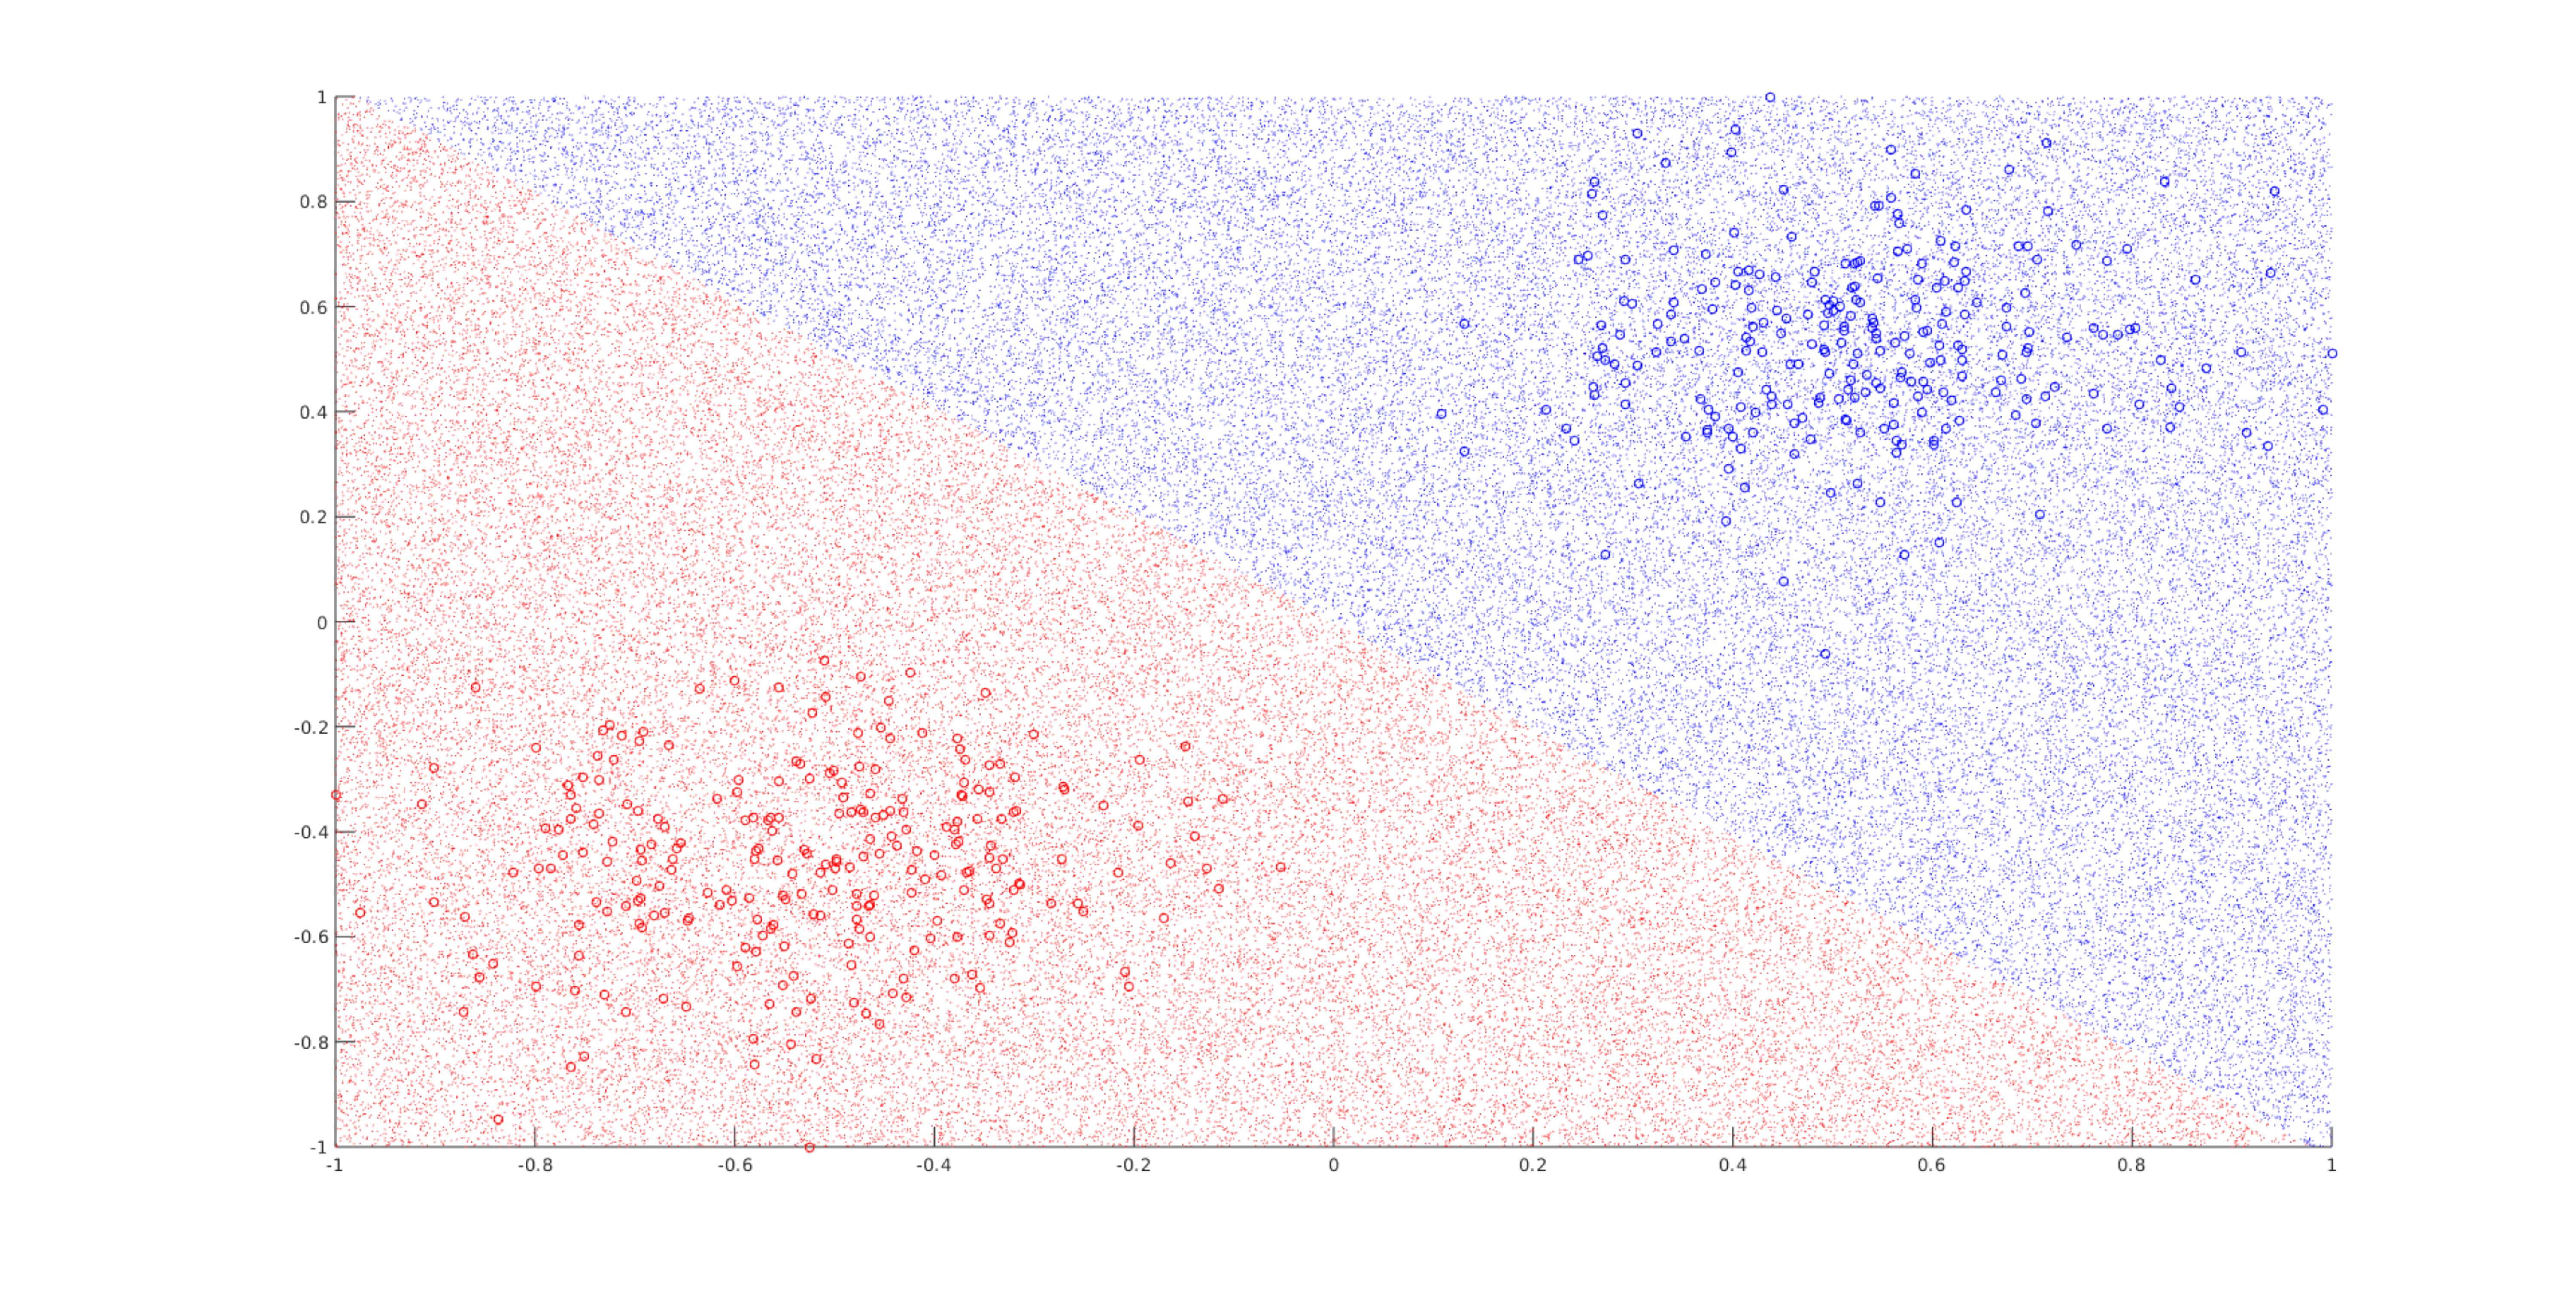
\includegraphics[width=\textwidth]{images/LinearBinaryClassifier}
\end{figure}
Utilizzando una funzione lineare, possiamo tracciare una retta
che divide due classi di punti bilanciati rispetto a tale asse. \\
Come nel caso della regressione lineare, nel caso i punti fossero non bilanciati
rispetto all'origine, si sarebbe dovuto introdurre un termine di bias.
\begin{figure}[H]
  \centering
  \includegraphics[width=\textwidth]{images/LinearBinaryClassifier2}
\end{figure}
Anche nel caso in cui i due gruppi di sample siano parzialmente coincidenti,
la funzione ottenuta sbaglia a assegnare la classe ai punti che si trovano piú vicini
rispetto al centro dell'altro cluster.
\begin{figure}[H]
  \centering
  \begin{subfigure}{0.30\textwidth}
    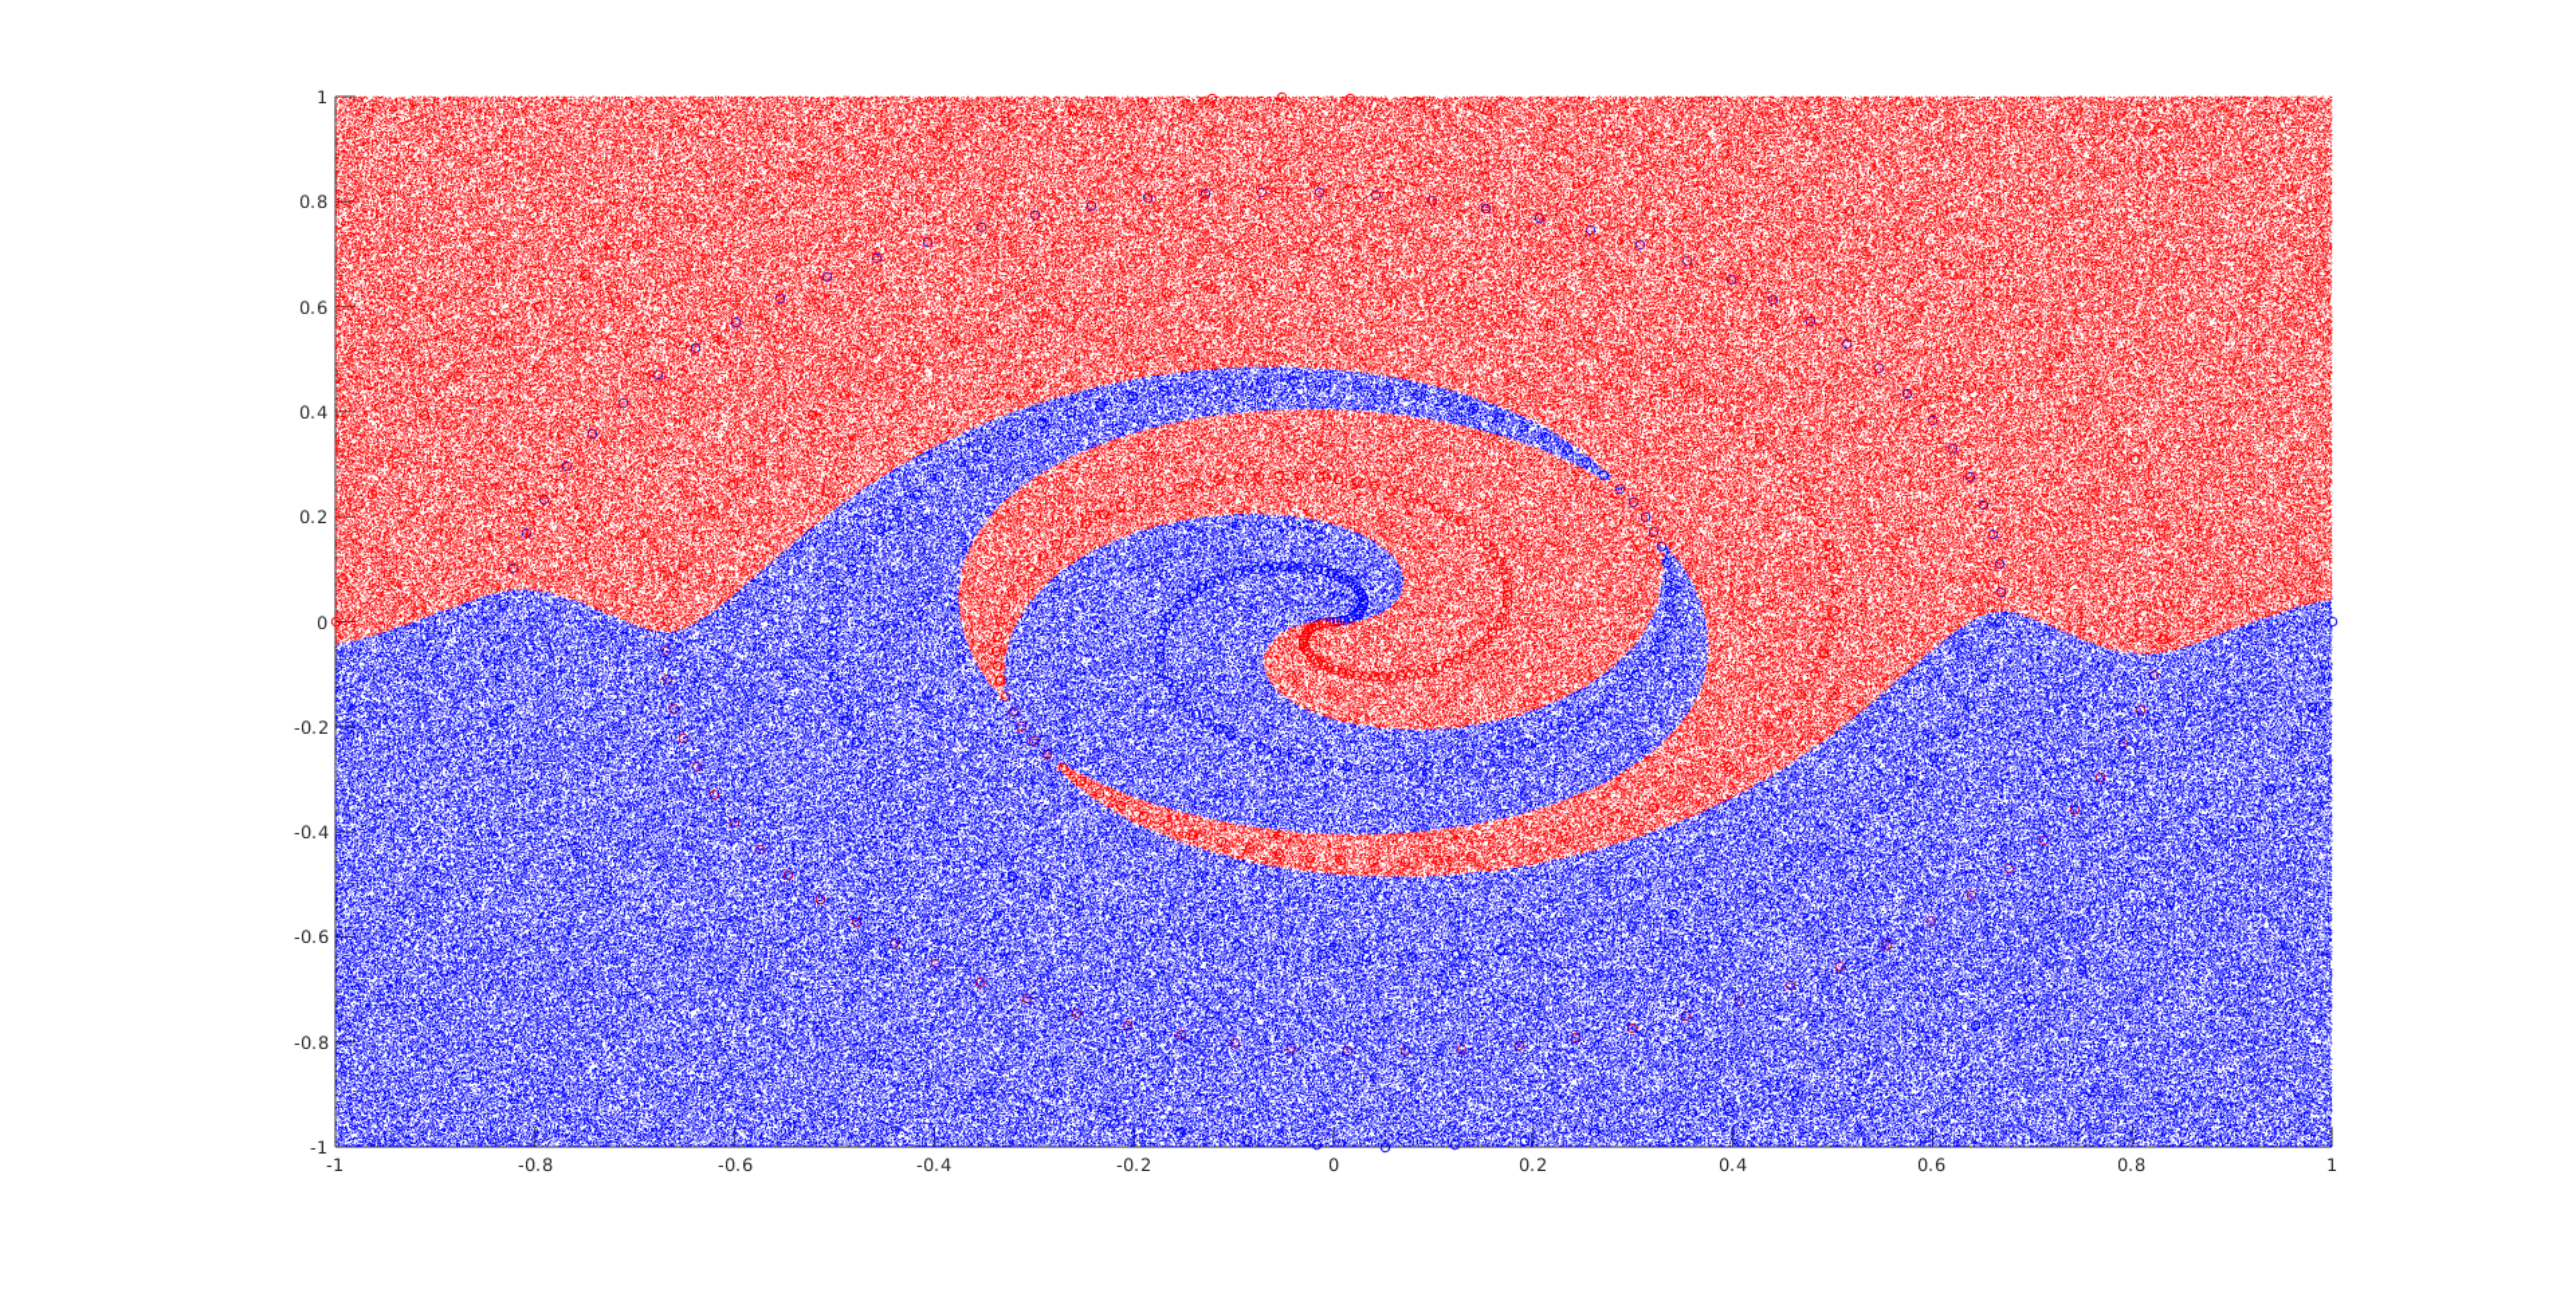
\includegraphics[width=\textwidth]{images/KernelBinaryLowGamma}
  \end{subfigure}
  \begin{subfigure}{0.30\textwidth}
    \includegraphics[width=\textwidth]{images/KernelBinaryMidGamma}
  \end{subfigure}
  \begin{subfigure}{0.30\textwidth}
    \includegraphics[width=\textwidth]{images/KernelBinaryHighGamma}
  \end{subfigure}
\end{figure}
Utilizzando un classificatore a kernel, possiamo classificare anche punti che non sono
bilanciati rispetto a una ideale retta che li divida.
Qui si hanno tre classificatori al variare di $\gamma$, da sinistra verso destra:
$\gamma = 0.1, \gamma = 1, \gamma = 10$.
Come si puó notare, il classificatore per gamma molto basso non riesce a classificare
correttamente tutti i sample, avendo bisogno di una funzione piú complessa.
Aumentado $\gamma$ si ottiene invece uno classificatore piú preciso, da notare che
il classificatore "intermedio", nonostante riesca a classificare correttamente tutti i punti,
presenta delle imperfezioni nella sua forma che possono causare una misclassificazione di eventuali
punti presenti nelle zone deformate.

\newpage
\section{Classificatore multiclasse A.V.A.}
Per classificare in piú classi, utilizziamo la tecnica ALL VS ALL, esiste anche un'altra tecnica, la ONE VS ALL che non tratteremo in questa relazione. \\
La tecnica AVA consiste nel trasformare il problema in uno o piú problemi di binary classification in modo da riutilizzare la conoscenza acquisita precedentemente.
$$
  n_p = {c \choose 2} \qquad n_p = \text{numero di problemi} \qquad c = \text{numero di classi}
$$
La classificazione di un punto consiste nell'utilizzare tutti i classificatori in sequenza e successivamente
decidere l'appartenenza del punto sulla base di una votazione a maggioranza di tutti i sottoclassificatori.
\begin{figure}[H]
  \centering
  \begin{subfigure}{0.48\textwidth}
    \includegraphics[width=\textwidth]{images/Multiclass_linear}
  \end{subfigure}
  \begin{subfigure}{0.48\textwidth}
    \includegraphics[width=\textwidth]{images/Multiclass_linear_fails}
  \end{subfigure}
\end{figure}
Nel caso di cluster di punti separabili linearmente (immagine a sinistra), l'approccio lineare permette
la loro corretta classificazione. \\
Nel caso presentato a destra, invece, il classificatore lineare non riesce a separare correttamente i cluster,
non potendo dividere i cluster posizionati lungo lo stesso raggio.
\begin{figure}[H]
  \centering
  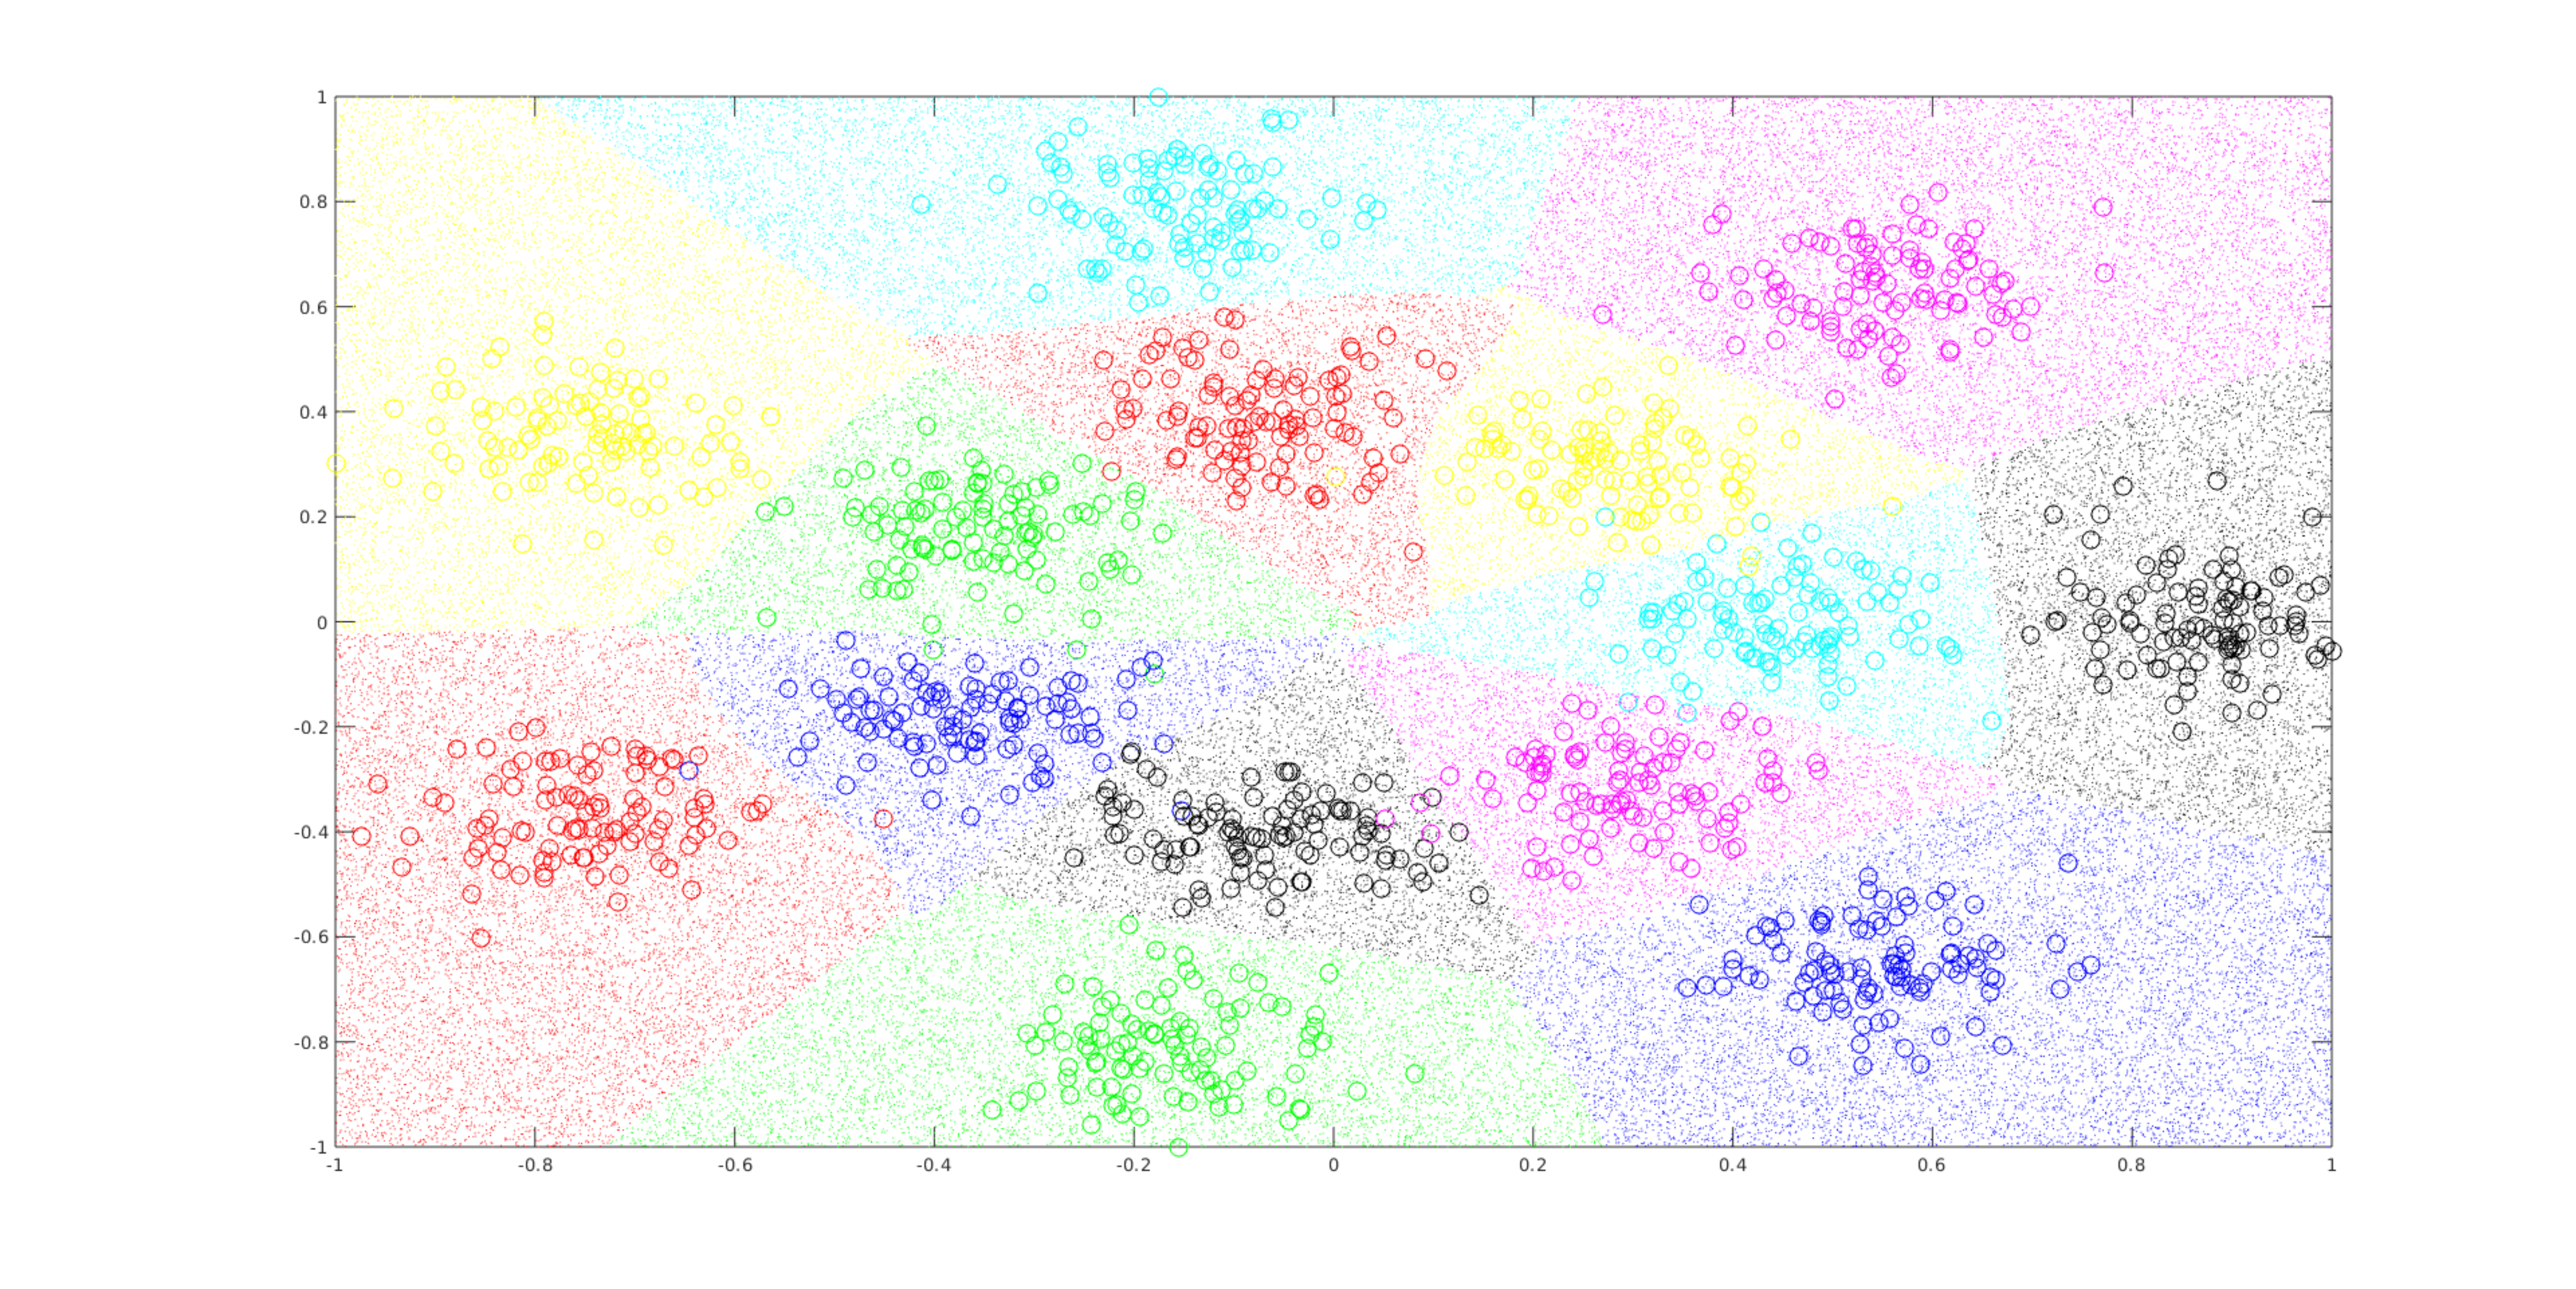
\includegraphics[width=\textwidth]{images/KernelAVA}
\end{figure}
Qui, utilizzando classificatori a kernel, si visualizzano le zone relative a 7 classi rappresentate dai 7 diversi colori. \\
Si evidenzia la forma non lineare delle zone risultanti. \\
Alcuni sample particolarmente distanti dal cluster piú vicino, sono stati classificati erroneamente.
Ad esempio, nel cluster di punti rossi in basso a sinistra é presente un sample blu.

\end{document}
